\subsubsection{最大流}

\begin{itemize}

\item \textbf{判断一条边是否必定满流}

在残量网络中跑一遍Tarjan, 如果某条满流边的两端处于同一SCC中则说明它不一定满流. (因为可以找出包含反向边的环, 增广之后就不满流了.)

\end{itemize}

\subsubsection{最小割}

首先牢记最小割的定义: 选权值和尽量小的一些边, 使得删除这些边之后$s$无法到达$t$.

\begin{itemize}

\item \textbf{最小割输出一种方案}

在残量网络上从$S$开始floodfill, 源点可达的记为$S$集, 不可达的记为$T$, 如果一条边的起点在$S$集而终点在$T$集, 就将其加入最小割中.

\item \textbf{最小割的可行边与必须边}

\begin{itemize}
	\item 可行边: 满流, 且残量网络上不存在$u$到$v$的路径, 也就是$u$和$v$不在同一SCC中. (实际上也就是最大流必定满流的边.)

	\item 必须边: 满流, 且残量网络上$S$可达$u$, $v$可达$T$.
\end{itemize}

\item \textbf{字典序最小的最小割}

直接按字典序从小到大的顺序依次判断每条边能否在最小割中即可.

如果一条边是可行边, 我们就需要把它删掉, 同时进行退流, $u\to s$和$t\to v$都退掉等同于这条边容量的流量.

退流用Dinic实现即可.

\end{itemize}

\subsubsection{费用流}


\subsubsection{上下界网络流}

\textbf{有源汇上下界最大流}

新建超级源汇$S', T'$, 然后如图所示转化每一条边.

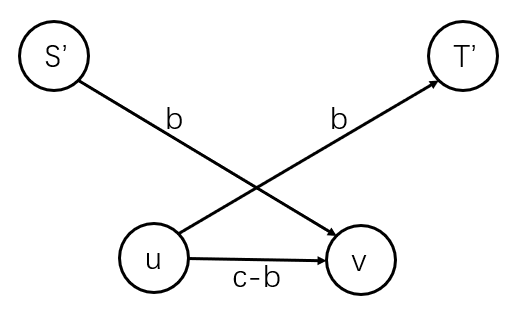
\includegraphics[scale = 0.5]{../src/graph/上下界网络流.png}

然后从$S'$到$S$, 从$T$到$T'$分别连容量为正无穷的边即可.

因为附加边实际上算了两次流量, 所以最终答案应该减掉所有下界之和.

\textbf{有源汇上下界最小流}

按照上面的方法转换后先跑一遍最大流, 然后撤掉超级源汇和附加边, 反过来跑一次最大流退流, 最大流减去退掉的流量就是最小流.

\textbf{无源汇上下界可行流}

转化方法和上面的图是一样的, 只不过不需要考虑原有的源汇了.

在新图跑一遍最大流之后检查一遍辅助边, 如果有辅助边没满流则无解, 否则把每条边的流量加上$b$就是一组可行方案.

\subsubsection{常见建图方法}

\begin{itemize}

\item \textbf{最大流/费用流}

流量不是很多的时候可以理解成很多条路径, 并且每条边可以经过的次数有限.

\item \textbf{最小割}

常用的模型是\textbf{最大权闭合子图}. 当然它并不是万能的, 因为限制条件可以带权值.

\begin{enumerate}

\item 如果某些点全部在$S$集或者$T$集则获得一个正的收益

把这个条件建成一个点, 向要求的点连$\infty$边, 然后$s$向它连$\infty$边. (如果是$T$集就都反过来)

那么如果它在$S$集就一定满足它要求的点都在$S$集, 反之如果是$T$集亦然.

\item 如果两个点不在同一集合中则需要付出代价

建双向边, 那显然如果它们不在同一集合中就需要割掉中间的边, 付出对应的代价.

\item 二分图, 如果相邻的两个点在同一集合则需要付出代价

染色后给一半的点反转源汇, 就转换成上面的问题了.

\end{enumerate}

\end{itemize}

\subsubsection{例题}

\begin{itemize}

% \item 最大流



% \item 最小割

% \begin{enumerate}

% \item 切糕

% \end{enumerate}

\item 费用流

\begin{enumerate}

\item 序列上选和尽量大的数, 但连续$k$个数中最多选$p$个.

费用流建图, 先建一条$n+1$个点的无限容量的链表示不选, 然后每个点往后面$k$个位置连边, 答案是流量为$p$的最大费用流. 因为条件等价于选$p$次并且每次选的所有数间隔都至少是$k$.

\item 还要求连续$k$个数中最少选$q$个.

任选一个位置把图前后切开就会发现通过截面的流量总和恰为$p$. 注意到如果走了最开始的链就代表不选, 因此要限制至少有$q$
的流量不走链, 那么只需要把链的容量改成$p - q$就行了.

\end{enumerate}

\end{itemize}